\documentclass[letterpaper,10pt]{article}

\usepackage[english]{babel}
\usepackage[utf8]{inputenc}
\usepackage{amsmath}
\usepackage{graphicx}
\usepackage[colorinlistoftodos]{todonotes}
\usepackage[top=1in, bottom=1in, left=1in, right=1in]{geometry}
\usepackage[small]{titlesec}

\newcommand{\bes}{\begin{equation*}}
\newcommand{\ben}[1]{\begin{equation}\label{#1}}
\newcommand{\ees}{\end{equation*}}
\newcommand{\be}{\begin{equation}}
\newcommand{\ee}{\end{equation}}

\newcommand{\bm}[1]{% inline column vector
	\begin{bmatrix}#1\end{bmatrix}%
}

\begin{document}

\begin{flushright}
{\Large Josh Bevan - HW6 Q5 - CS450}
\end{flushright}
\vskip -0.1in
\hrule
\vskip 0.3in

\textit{Consider the ODE $y'=-5y$ with initial condition $y(0)=1$. We will solve this ODE numerically using a step size of $h=0.5$.}

\section*{Are solutions to this ODE stable? Explain.}
Solutions to this ODE are asymptotically stable. Consider Figure 1 which plots solutions of $y'$ for the initial condition $y(0)=1$ as well as a number of other initial conditions. It is clear that even  solutions with perturbations to their initial value converge back to the true solution.
\begin{figure}[!htb]
\centering
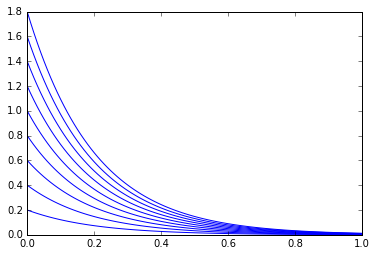
\includegraphics[width=0.6\textwidth]{stable.PNG}
\caption{Plot of solutions of $y'$ for differing initial conditions.}
\end{figure}

\section*{Is Euler's method stable for this ODE using this step size? Explain.}
Euler's method is not stable for this ODE and step size. Recall that for problems of the type $y' = \lambda y$, with fixed step size $h$, a stable step size must satisfy $h \leq -\frac{2}{\lambda}$. In this case $\lambda=-5$, so  $h \leq -\frac{2}{-5}=0.4$; we can see that our step size does not satisfy the inequality and therefore Euler's method with this step size will be unstable.

\section*{Compute the numerical value for the approximate solution at $t=0.5$ given by Euler's method. Show your work.}
\be y(0.5) \underset{Euler, \,h=0.5}{=} hy'(0)+y(0) = 0.5(-5y(0))+y(0) = 0.5(-5)+1 =-2.5+1 = -1.5 \ee

\section*{Is the backward Euler method stable for this ODE using this step size? Explain.}
Backward Euler is stable for this ODE using this step size. Recall that for problems of the type $y' = \lambda y$, with fixed step size $h$, a stable step size must satisfy:
\be \lvert \frac{1}{1-h\lambda} \rvert \leq 1, \; \text{in our case:} \;  \lvert \frac{1}{1-0.5(-5)} \rvert =  \lvert \frac{1}{3.5} \rvert \leq 1 \ee
so backward Euler is stable for this step size.

\section*{Compute the numerical value for the approximate solution at $t=0.5$ given by the backward Euler method. Show your work.}
\be y(0.5) \underset{backEuler, \,h=0.5}{=} hy'(0.5)+y(0) = 0.5(-5y(0.5))+1 \ee
solving for $y(0.5)$:
\be y(0.5) = -2.5y(0.5)+1 \rightarrow 3.5y(0.5)=1 \rightarrow y(0.5) = 1/3.5 \approx 0.2857\ee

\end{document}